\chapter{VPN and VLANs}
\label{ch:vpn_vlan}

%----------------------------------------------------------------------------------------

\section{VPN}
\begin{figure}[h]
    \centering
    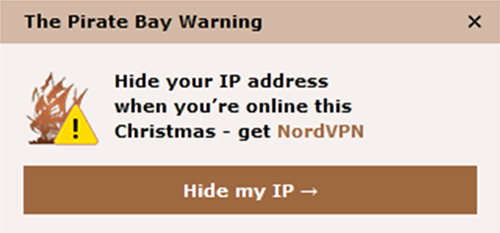
\includegraphics[scale=0.5]{img/tpb_vpn.png}
    \decoRule
    \caption{The Pirate Bay VPN message. They even got a nice discount this year.}
    \label{fig:tpb_vpn}
\end{figure}

Every time we visit a torrent website we are welcomed by a message showing our IP address and telling us that our ISP is seeing everything we do, yada, yada, yada, and they basically want us to buy this or that VPN (figure \ref{fig:tpb_vpn}). But what is a VPN, and why is it important?

Let us assume that we have two computers, A and B, that want to connect to the Internet (the cloud in figure \ref{fig:vpn}), and we also want to have a private channel between these two devices. This channel has to be private, meaning that an attacker shall not be able to see what is inside. This is what is normally called a \textbf{VPN}, or \textbf{Virtual Private Network}.

\begin{figure}[h]
    \centering
    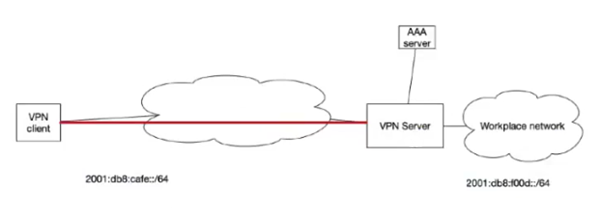
\includegraphics[scale=0.7]{img/vpn.png}
    \decoRule
    \caption{Diagram of a simple VPN.}
    \label{fig:vpn}
\end{figure}
 
Someone might ask what is the difference between VPN and HTTPS. Surprisingly, the answer is that there is no difference except for the fact that in a HTTPS connection we use HTTP, while in a VPN we can transfer anything.

There are a zillion ways to make a VPN, although one size does \textit{not} fit all. What we must ask ourselves is whether we want a VPN that transfers IP frames, or one that uses Ethernet frames, or another running at application level: they are all called VPNs, but they reflect different ideas and different ways of working.

We should be acquainted with VPNs and always use them: everybody should have a trusted VPN server somewhere (possibly hosted by ourselves). There are many VPN servers offered in the cloud, but this is clearly not a good idea because we would have to trust another system, and hell, we cannot even trust ourselves, so why should we trust somebody else to be able to decrypt everything we send? Nonetheless, paying a few bucks per month in order to have a VPN server somewhere is still better than not having it at all.

%-------------------------------------------

\subsection{Layer 2 VPN}
Let us start with the lowest level: suppose that we want to transfer \textbf{whole Ethernet dataframes}. This might be useful when we have an office in one room (like a laboratory) and another computer several rooms away (could also be located in a different building and/or city), and we want to use the system like we were physically in that office - meaning that we would like to use the lowest level, link-local protocols. We must somehow pretend to be in the same physical network as the office, and the only possible way to do this is to transfer whole Ethernet frames from one place to another.

Generally, we have a number of ways to achieve this, but we need to find an easy, fast and encrypted solution (in order to maintain confidentiality and integrity). For this reason we can find in a VPN all the issues related to authentication, authorization, encryption, secrecy, reliability, etc.

Suppose that we found a way to build our VPN. If we open a session between A and B (like a TCP stream), then on top of that TCP stream we put something that ensures authentication, authorization, confidentiality, non repudiability and integrity, and on this channel (because at this point it is a channel) we can simply send packets. The content of the packets can be anything, so even a full Ethernet frame - nobody cares, as the only thing needed on the other side of the channel is something able to get those frames and slam them in an Ethernet port as they are.
 
All variations and complications of VPNs derive from this general framework: we have a process on device A that grabs something, encapsulates it into something secure and then transfers it to the other side, where it is decapsulated and used like it were something else.
 
At low level, however, sending Ethernet frames is \textit{not} the most flexible and elegant thing to do, because in a local network we assume to have a large bandwidth and thus the end result of transferring layer 2 packets is that our secure channel is overburdened with packets that actually are not interesting for the other side.

This means that we need to filter those frames that would not usually be found in a common switched network. Suppose that we know what are the Ethernet numbers on the other side, and we filter Ethernet frames based on their destination address; it is slightly more than what a switch would do. Also mind that a VPN normally is made of a VPN server and a VPN client, meaning that it does not realize a point-to-point channel between two devices (although it could). Usually, the VPN server acts as a concentrator to gather VPN endpoints from a number of clients, and it is also connected to an AAA server (because it will be served by something like 802.1X).

%-------------------------------------------

\subsection{Layer 3 VPN}
Transferring Ethernet frames is not something that many users want to do. An option is to transfer IP datagrams instead, moving up from layer 2 to layer 3. In this case the VPN server acts like a router, instead of a switch.

%-------------------------------------------

\subsection{Application level VPN}
The third option  is to transfer directly \textbf{application level streams}, which are much like HTTPS. Security-wise, at this level attackers have more options, but so do admins, who are more fine-grained about what their users can or cannot do (e.g. decide that user A can use services Z and Y, while user B can use Z but not Y).

In order to create a VPN at application level we can use TLS on top of TCP (although this is not the only option). In this case we still have TCP’s vulnerabilities, and we would only protect the VPN’s content, not the VPN itself.
 
Another problem is that TCP has the bad habit of trying to figure out what is the optimal bandwidth of the channel, and then tweaking its windows according to the channel occupancy (the infamous \textbf{congestion control}). While this feature is more or less what makes the Internet work, if we open a TCP connection over a VPN that is using TCP (see figure \ref{fig:tcp_in_tcp}) we get a highly unstable system, as the inner and outer TCP layers would have the same speed.

\begin{figure}[h]
    \centering
    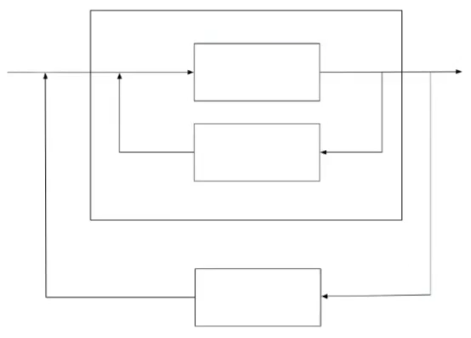
\includegraphics[scale=0.7]{img/tcp_in_tcp.png}
    \decoRule
    \caption{TCP over TCP is a bad idea.}
    \label{fig:tcp_in_tcp}
\end{figure}

An unstable system is unpredictable and is in for \textit{huge} oscillations. From a network point of view, in order to make it work we would need a special TCP flavor for the outer or the inner layer. In the outer layer (the TCP on which the VPN has been built) it would affect the whole VPN (our data flow, too); in the inner, well, who is going to tell an application or our OS that they have to use a special TCP because their flow is going through a VPN? No one.

Given these huge performance issues, we cannot really use TCP for VPN. The solution is to use \textbf{UDP}, although in this case we have to cope with the fact that TLS is meant to run over TCP, not UDP, so we would need a special version of TLS or another layer on top of UDP in order to make it session-oriented. And while this seems complicated, it is what is actually done in practice. Mind that using UDP means that the VPN will open a number of ports on our NAT, so if we use a VPN we should also use a firewall, otherwise our clients might be endangered.

%-------------------------------------------

\subsection{VPN implementations}
There are many different VPN implementations; we will only see a few of them.

%----------------------

\subsubsection*{IPsec}
\textbf{IPsec} can be used as a VPN, as it works at IP level. Its basic idea is shown in figure \ref{fig:ipsec_vpn}.

\begin{figure}[h]
    \centering
    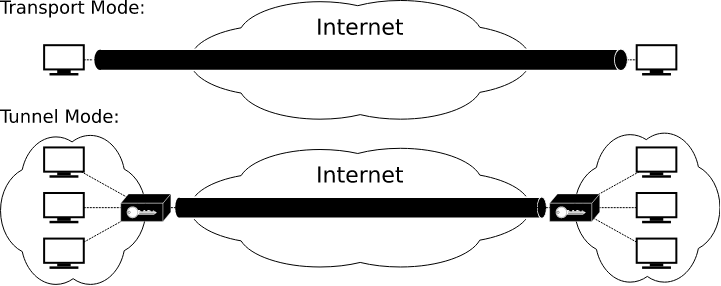
\includegraphics[scale=0.5]{img/ipsec_vpn.png}
    \decoRule
    \caption{IPsec transport and tunnel modes.}
    \label{fig:ipsec_vpn}
\end{figure}

In transport mode we transfer layer 3 data, while in tunnel mode we transfer layer 2 data, meaning that it can be used as a VPN. The problem is that IPsec is extremely complicated, so basically nobody uses it for this. It is also \textit{not} NAT-friendly: if we have a NAT we would need to use IP-over-IP, (actually IPsec-over-IP), which is a nightmare.

%----------------------

\subsubsection*{OpenVPN}
An alternative to IPsec is \textbf{OpenVPN}, practically something that everybody uses. It is the classical protocol that is well-known, well-accepted and works - the good old trusted system. It is reliable and open source (we can install our server and then we can install any client, even for our phone, and access our stuff).

%----------------------

\subsubsection*{Wireguard}
\textbf{Wireguard} is a next generation VPN system. It is much, \textit{much} simpler (implementation-wise) than OpenVPN, because it does not support backwards compatibility and thus avoids being bloated by code that is there to ensure that newer versions of the client work with older versions of the server. This also means that we have to be careful when installing new versions, and we have to remove, for example, blacklisted versions of protocols, etc. (in other words we must keep it constantly updated).

The end result is a system that is smaller sized and more easily checked. Mind that a VPN is an extremely critical piece of code, like a kernel extension: it must work and it must be bug and vulnerability free, so the smaller the code base, the easier the audit of the system.

Moreover, Wireguard uses a different approach for user authentication and routing, which is something that must be taken into account while setting it up. While OpenVPN is extremely traditional in a networking sense (the client talks to the server, the server talks back to the client, in a classic star topology, and routing wise it just uses the Internet), Wireguard uses \textbf{cryptokey routing}, which associates a private key with the user's identity, meaning that we will not be addressed with an IP, but with our identity (effectively decoupling it from the IP address).

Note that this feature also allows users to directly communicate with each other and go peer-to-peer, making Wireguard way faster than other VPNs (for example, while a VPN normally takes out about 80\% of the available bandwidth, Wireguard is able to squeeze a lot more).

The caveat is that Wireguard is kinda new, so its documentation is not yet widespread. Still, it looks like an extremely promising tool, especially because it is natively included in the Linux kernel - meaning that performance will be even greater, and with time it will be more widely spread and accepted.

%----------------------------------------------------------------------------------------

\section{VLANs}
Suppose that we have to lay down a network in a building, but we have no idea about who is going where, and maybe not even how it is going to be used.

\vspace{0.5em}

\emph{Example} The network of the department of Information Engineering at the University of Florence encompasses a whole one floor of the building, and the network setup is a nightmare because some rooms are offices, some are labs, and some are both (so they need to access to normal Internet and the internal lab network). To add to this mess, the administration also has the bad habit of moving people around the offices or changing their roles.

\vspace{0.5em}
 
We would like the network to be functional without sacrificing security. Usually, we either have control over the physical network or we cannot secure a proper separation of the internal networks - so how do we do this without knowing in advance who will be sitting where and what will do?
 
We already know that through the coherent use of authentication and access control (e.g. 802.1X) we can make sure that only authorized users can plug their cable into an outlet and use the network. But what if we need to give access to the same plug to a student and a professor, indifferently? We could give them different priorities using the 802.1X protocol, and then set up what is called a \textbf{VLAN}, or \textbf{Virtual LAN}, which from the point of view of network security is mandatory.
 
A VLAN is nothing more than a nifty name for a technology deeply rooted into 800.3\footnote{It is not exactly 802.3, but actually 800.1 applied to 802.3; we could use it in any 802 network, but additional restrictions would apply.}; the most common situation is to use it over Ethernet.
 
In other words a VLAN is a way - any way - of splitting a physical network into many virtual physical networks, ensuring \textbf{separation} between different virtualized networks. Mind that we are not talking about software defined networking (which is a completely different concept and idea); VLANs are more practical and well-oiled, and have also been standardized under the IEEE 802.1Q standard.
 
802.1Q states a rather simple, but powerful (and dangerous) concept. In this standard the role of enforcing separation between flows that are not part of the same virtual network falls to the \textbf{switch}. Mind that every time we give a device an additional bit of responsibility, we are making them more vulnerable, and they become a point of attack. VLANs in particular are an extremely sensitive point because switches tend to be quite cheap and not very well-protected.

%-------------------------------------------
\subsection{VLAN tagging system}
Suppose that the switch works as intended. Virtual LANs are based on the simple idea of assigning colors to cables and ports: every port of the switch has a color, different ports can have the same color, and only ports with the same color are enabled to talk to each other. From the switch's point of view ports of the same color will have a common MAC address translation table, and different tables belonging to different colors are completely separated.

\vspace{0.5em}

\emph{Example} Let us say that a packet arrives from a pink cable, and we do not know the destination MAC address, so we have to send the packet in broadcast. The data will not be sent to every port, but only to those of the same color (pink). If the packet had the MAC address of another machine attached to the switch - but to a different color – then it would have been dropped.

\vspace{0.5em}

The color of a packet is embedded into the Ethernet frame, and contained into a header prepended to the Ethernet size and payload (figure \ref{fig:vlan_tag}), although it can also be used in different technologies, like Wi-Fi.

The 1Q header is made of 4 bytes: 16 bits for the TPID placeholder (its value is normally \texttt{8100}, chosen so as not to be a valid number for an Ethernet frame, because when we receive an Ethernet frame we do not know if we have a 1Q header or not) and 2 bytes for priorities (3 bits) and the drop-eligible indicator (1 bit, indicating the dropping priority in case of congestion). The remaining 12 bits are the VLAN indicator or identifier; we could have more than 4000 VLANs on the same switch.

\begin{figure}[h]
    \centering
    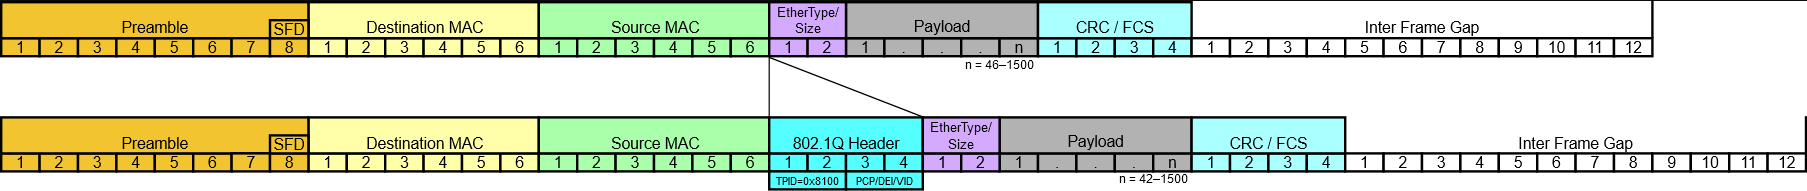
\includegraphics[scale=0.25]{img/vlan_tag.png}
    \decoRule
    \caption{Insertion of 802.1Q tag in an Ethernet frame.}
    \label{fig:vlan_tag}
\end{figure}
 
The catch here is that it is not obvious \textit{who} decides the tags, and this is a fundamental issue since they indicate who can and who cannot be trusted.

Suppose that we have a computer attached to a VLAN. We have authenticated it, so we trust both the computer and the user, right? Wrong. We must not - cannot - fully trust the user, even if it is authenticated, nor the computer, as it might contain malware.
 
At this point we can choose between two different policies: trusting the device and allowing it to attach the tags (the most permissive policy), or let the switch tag the packets.

If the tags are applied by the switch, one might argue that they are not needed since the switch could just send packets to the intended devices directly. This is not wrong, but when there are multiple switches tags become mandatory in order for the VLAN to work, because ports of the same colors might very well be scattered among different switches. Sometimes the final switch will remove the tags, making the VLAN completely transparent to its users.

The IEEE 802.1ad extension adds the option to have tags inside other tags, effectively introducing a \textbf{multiple layer tagging system} in which the outer tag has a different TPID; normally, it is only used in large organizations.

There is another thing that is \textit{not} obvious, and it is how to set up the communication and meaning of tags between different switches. Since this is not covered in the standard, a number of proprietary standards have been proposed.

%-------------------------------------------
\subsection{Multiple VLANs}
When a user is connected to more than one VLAN at the same time, to the same switch, they do not have to remove or change the tags, because their device must be able to recognize that there are two (or more) VLANs, and hopefully it automatically configures two separated VLAN ports with two different (maybe, but is not relevant) MAC addresses and two different IP addresses. Normally, it works.

%-------------------------------------------
\subsection{Performance}
VLANs introduce slightly \textbf{more latency}, especially if the switches are not performing well (hopefully not due to the tags, otherwise it means that we got some really cheap devices). The other catch is that by introducing 32 more bits (4 bytes) in the frame we are actually \textbf{decreasing} the \textbf{payload size} - that is, if we want to keep the total frame size, otherwise we will have longer frames. The final result is that our useful throughput (the \textit{goodput}) is slightly lower - but hopefully we are not trying to squeeze the last bit from our connection (this would mean that the network is deeply underprovided and should be upgraded). Mind that bottlenecks at physical level are a sign of bad configuration.